
\documentclass[fleqn,addpoints]{exam}

\usepackage{graphicx}
\usepackage{booktabs}
\usepackage{float}
\usepackage{amsmath}
\usepackage{cancel}
\usepackage{polynom}
\usepackage{caption}
\usepackage{mdwlist}

\newcommand{\degree}{\ensuremath{^\circ}} 

\printanswers

\ifprintanswers 
\usepackage{2in1, lscape} 
\fi

\title{Math 115 \\ Homework 23}
\date{May 17, 2011}

\begin{document}

\maketitle

% \begin{figure}[H]
%   \centering
%   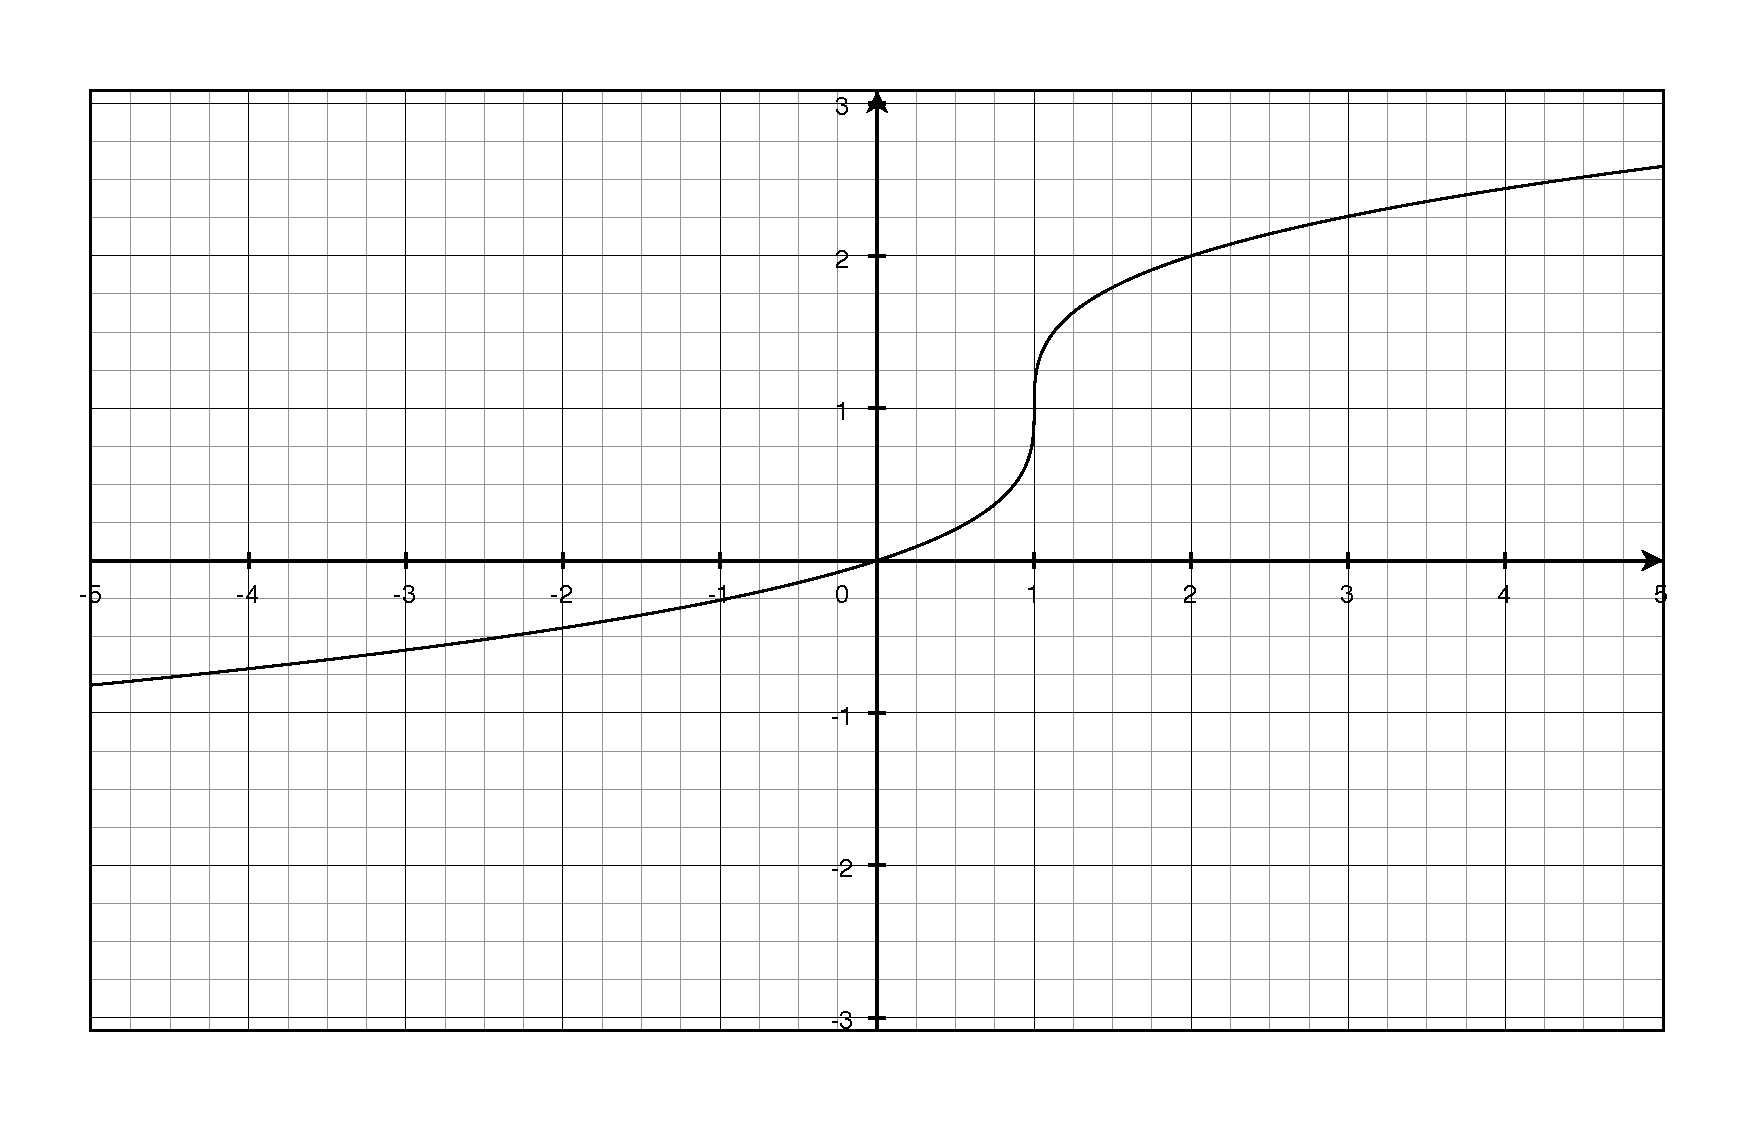
\includegraphics[scale=.3]{question7.eps}
%   \caption*{Question 7}
% \end{figure}

% \begin{tabular}{cc}
% \toprule
% period & amplitude \\
% \midrule
%   $\pi$ & $2$ \\
% \bottomrule
% \end{tabular}


\section{Homework}
\begin{itemize*}
  \item pp 418-421: 1-5, 11-15, 33-34, 39-40, 45-46, 51-54, 63-66, 76-77, 80, 82, 92, 94, 96-97
  \item pp 428-431: 15, 21, 25, 27, 49
\end{itemize*}

185 points

\section{Extra Credit}
\begin{itemize*}
  \item p. 420, question 99

\begin{solution}
\begin{figure}[H]
  \centering
  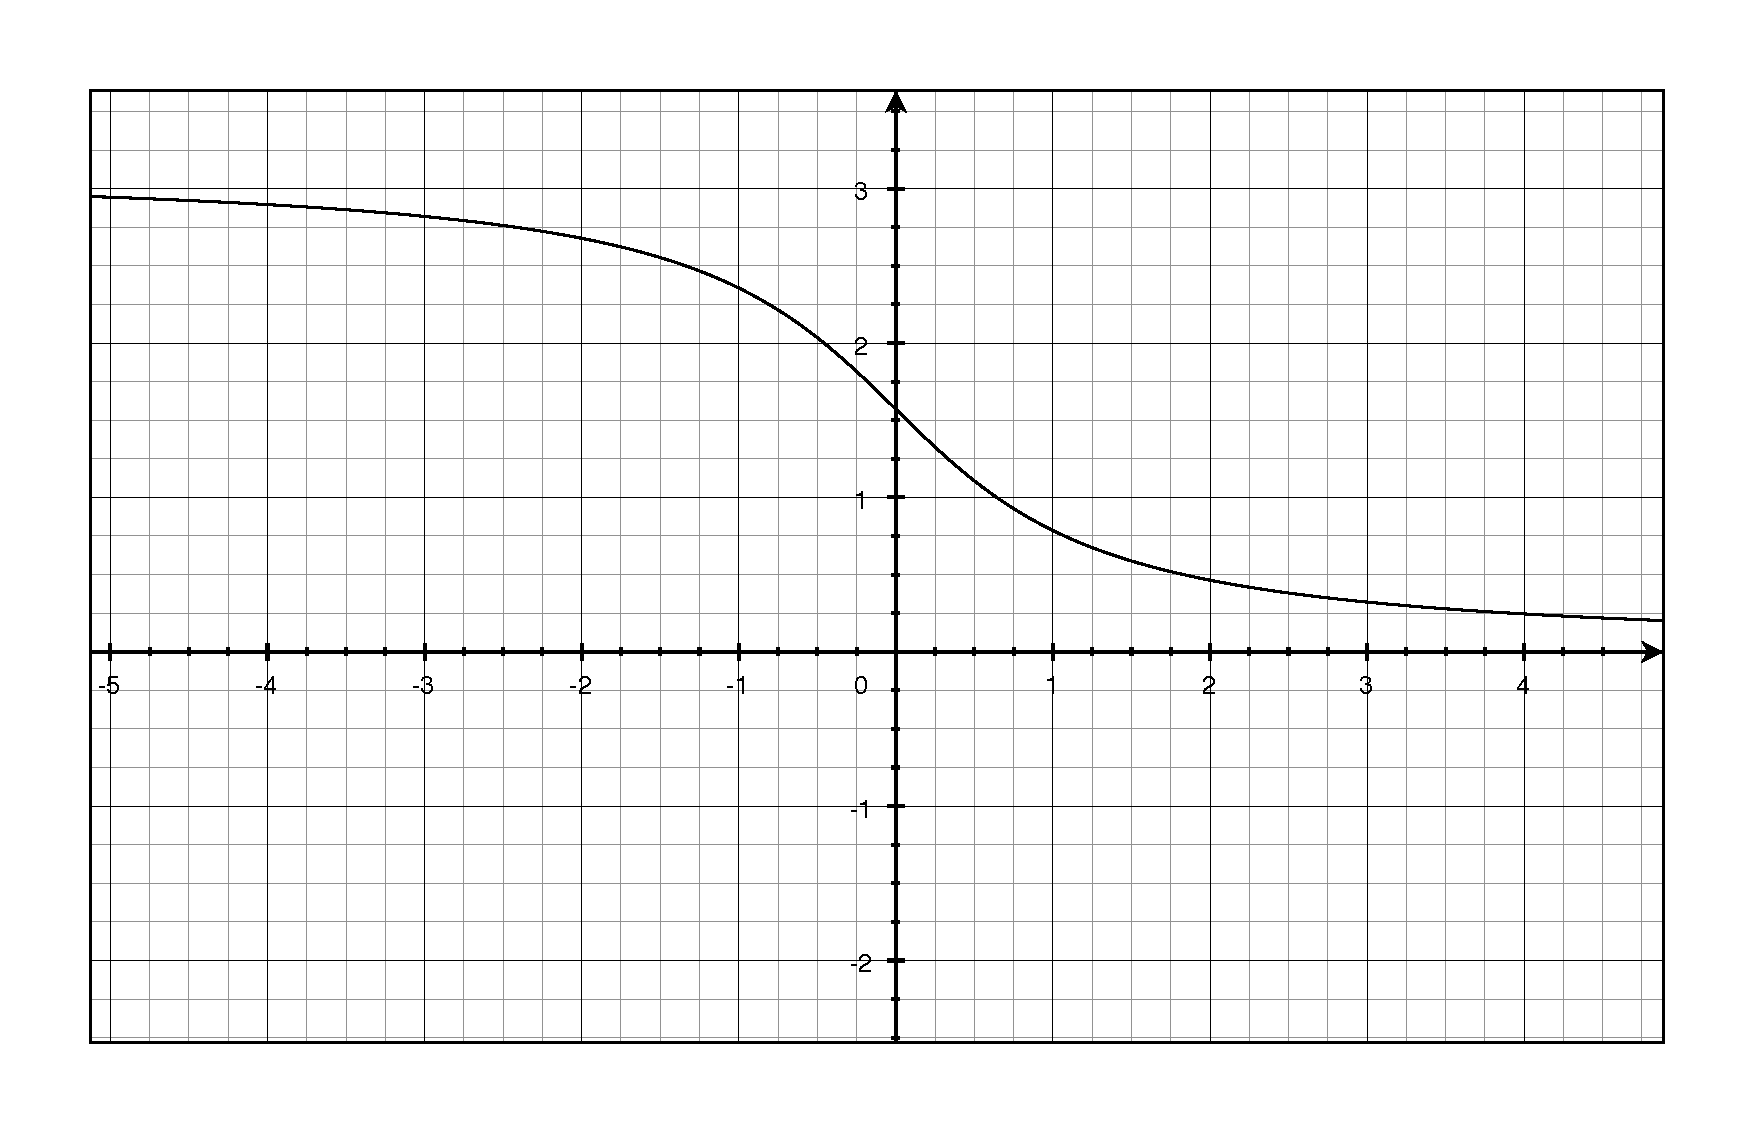
\includegraphics[scale=.3]{question_99.eps}
  \caption*{Question 99}
\end{figure}

\end{solution}

  \item p. 430, question 43

\begin{solution}
The length of the diagonal is $d = \sqrt{2 a^2} = a \sqrt{2}$.  

So 
\[
  \tan \theta = \frac{\cancel{a}}{\cancel{a} \sqrt{2}} = \frac{\sqrt{2}}{2}
\]

And:
\[
  \theta = \arctan \frac{\sqrt{2}}{2} = 35.3 \degree
\]

\end{solution}

\end{itemize*}

\ifprintanswers
\section{Pages 418-421}

\begin{description}

\item[1] 
\[
  \arcsin \frac{1}{2} = \frac{\pi}{6}
\]

\item[2] 
\[
  \arcsin 0 = 0
\]

\item[3] 
\[
  \arccos \frac{1}{2} = \frac{\pi}{3}
\]

\item[4] 
\[
  \arccos 0 = \frac{\pi}{2}
\]

\item[5] 
\[
  \arctan \frac{\sqrt{3}}{3} = \frac{\pi}{6}
\]

\item[11] 
\[
  \arccos \left( - \frac{1}{2} \right) = \frac{2 \pi}{3}
\]

\item[12] 
\[
  \arcsin \frac{\sqrt{2}}{2} = \frac{\pi}{4}
\]

\item[13] 
\[
  \arcsin \frac{\sqrt{3}}{2} = \frac{\pi}{3}
\]

\item[14] 
\[
  \arctan \left( - \frac{\sqrt{3}}{3} \right) = - \frac{\pi}{6}
\]

\item[15] 
\[
  \arctan 0 = 0
\]

\item[33] $\left(- \sqrt{3}, -\dfrac{\pi}{3}\right)$, $\left(- \dfrac{\sqrt{3}}{3}, \dfrac{\pi}{6}\right)$, 
  $\left(1, \dfrac{\pi}{4}\right)$

\item[34] $(-1, \pi)$, $\left( -\dfrac{1}{2}, \dfrac{2 \pi}{3} \right)$, $\left( \dfrac{\sqrt{3}}{2}, \dfrac{\pi}{6} \right)$

\item[39] 
\[
  \theta = \arcsin \frac{x+2}{5}
\]

\item[40] 
\[
  \theta = \arcsin \frac{x+1}{10}
\]

\item[45] 
\[
  \cos [ \arccos ( -0.1 ) ] = -0.1
\]

\item[46] 
\[
  \sin [ \arcsin ( -0.2 ) ] = -0.2
\]

\item[51] 
\[
   \cos(\arctan 2)) = \frac{\sqrt{5}}{5}
\]

\item[52] 
\[
   \sin \left( \arccos \frac{\sqrt{5}}{5} \right) = \frac{2\sqrt{5}}{5}
\]

\item[53] 
\[
   \cos \left (\arcsin \frac{5}{13} \right) = \frac{12}{13}
\]

\item[54] 
\[
   \csc \left( \arctan \left( - \frac{5}{12} \right) \right) = - \frac{13}{5}
\]

\item[63] 
\[
   \sin(\arccos x)) = \sqrt{1 - x^2}
\]

\item[64] 
\[
   \sec(\arcsin(x-1)) = \frac{1}{\sqrt{2x - x^2}}
\]

\item[65] 
\[
   \tan\left( \arccos \frac{x}{3} \right) = \frac{\sqrt{9-x^2}}{x}
\]

\item[66] 
\[
   \cot \left( \arctan \frac{1}{x} \right) = x
\]

\item[76] 
\begin{figure}[H]
  \centering
  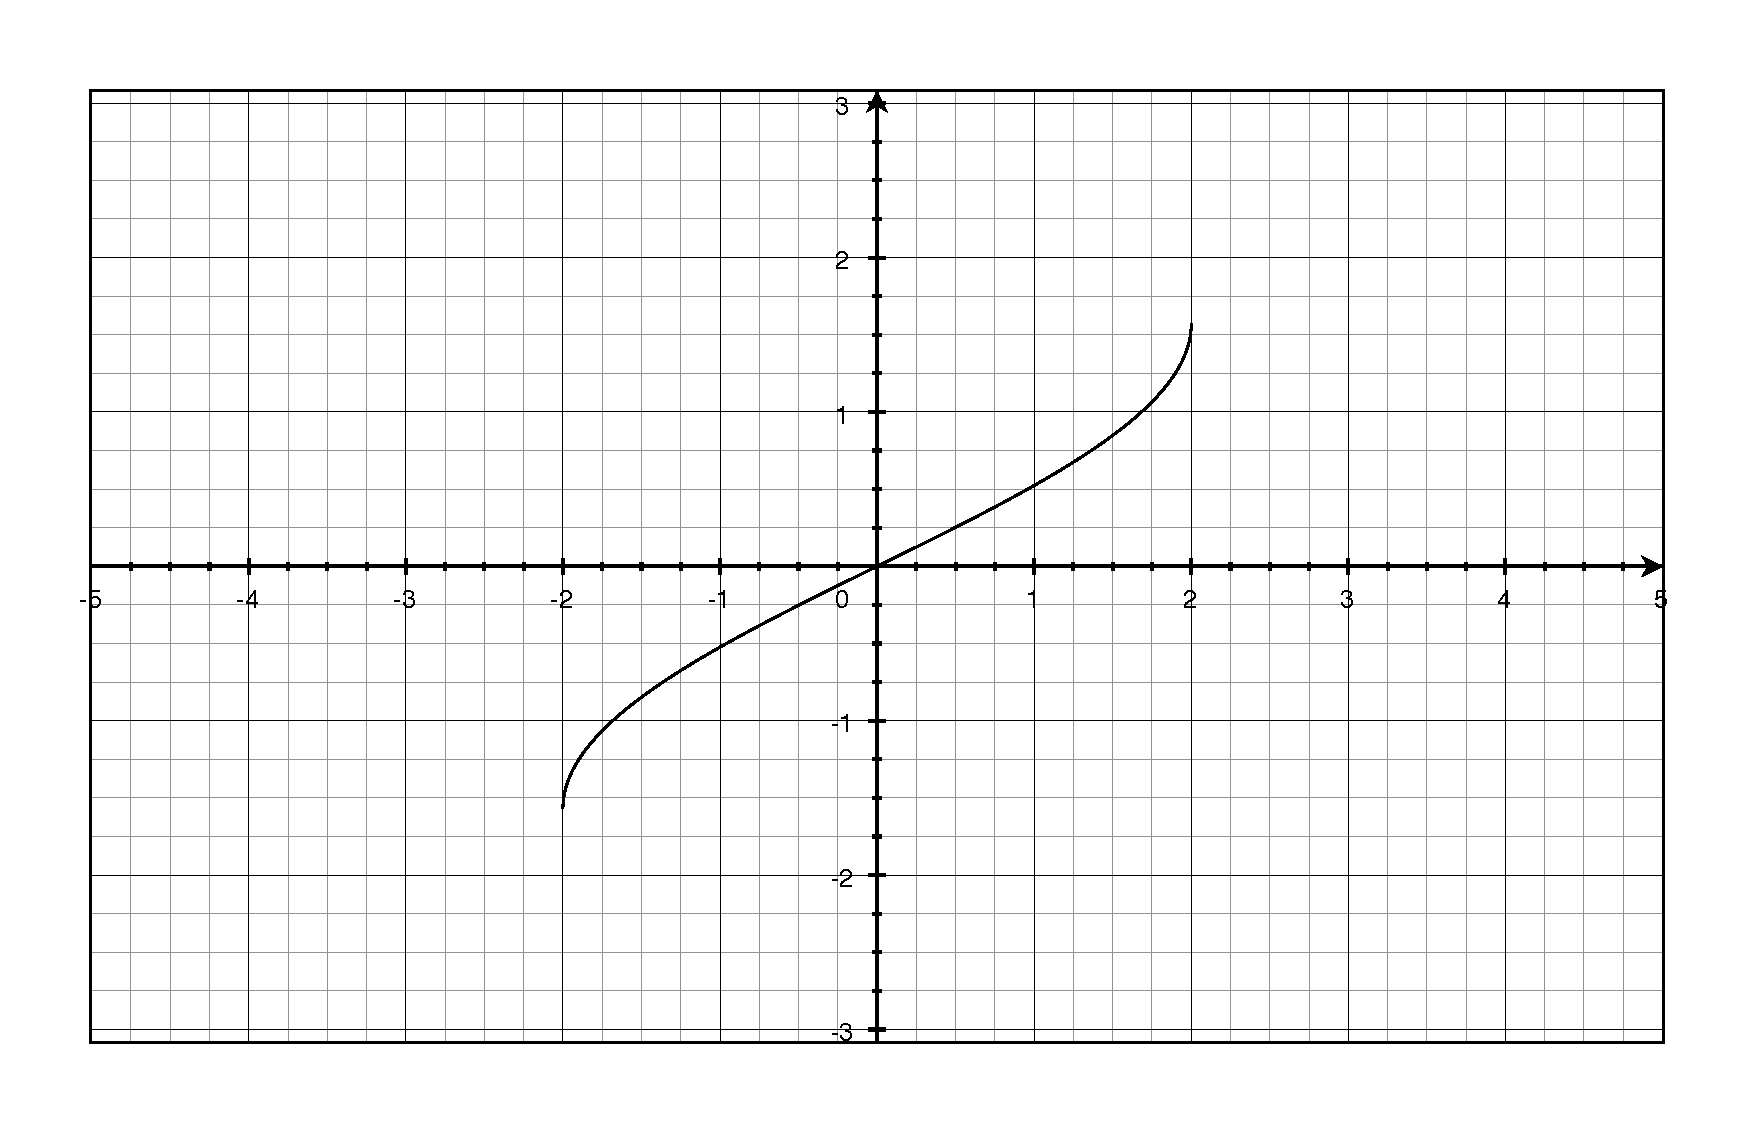
\includegraphics[scale=.3]{question_76.eps}
  \caption*{Question 76}
\end{figure}


\item[77] 
\begin{figure}[H]
  \centering
  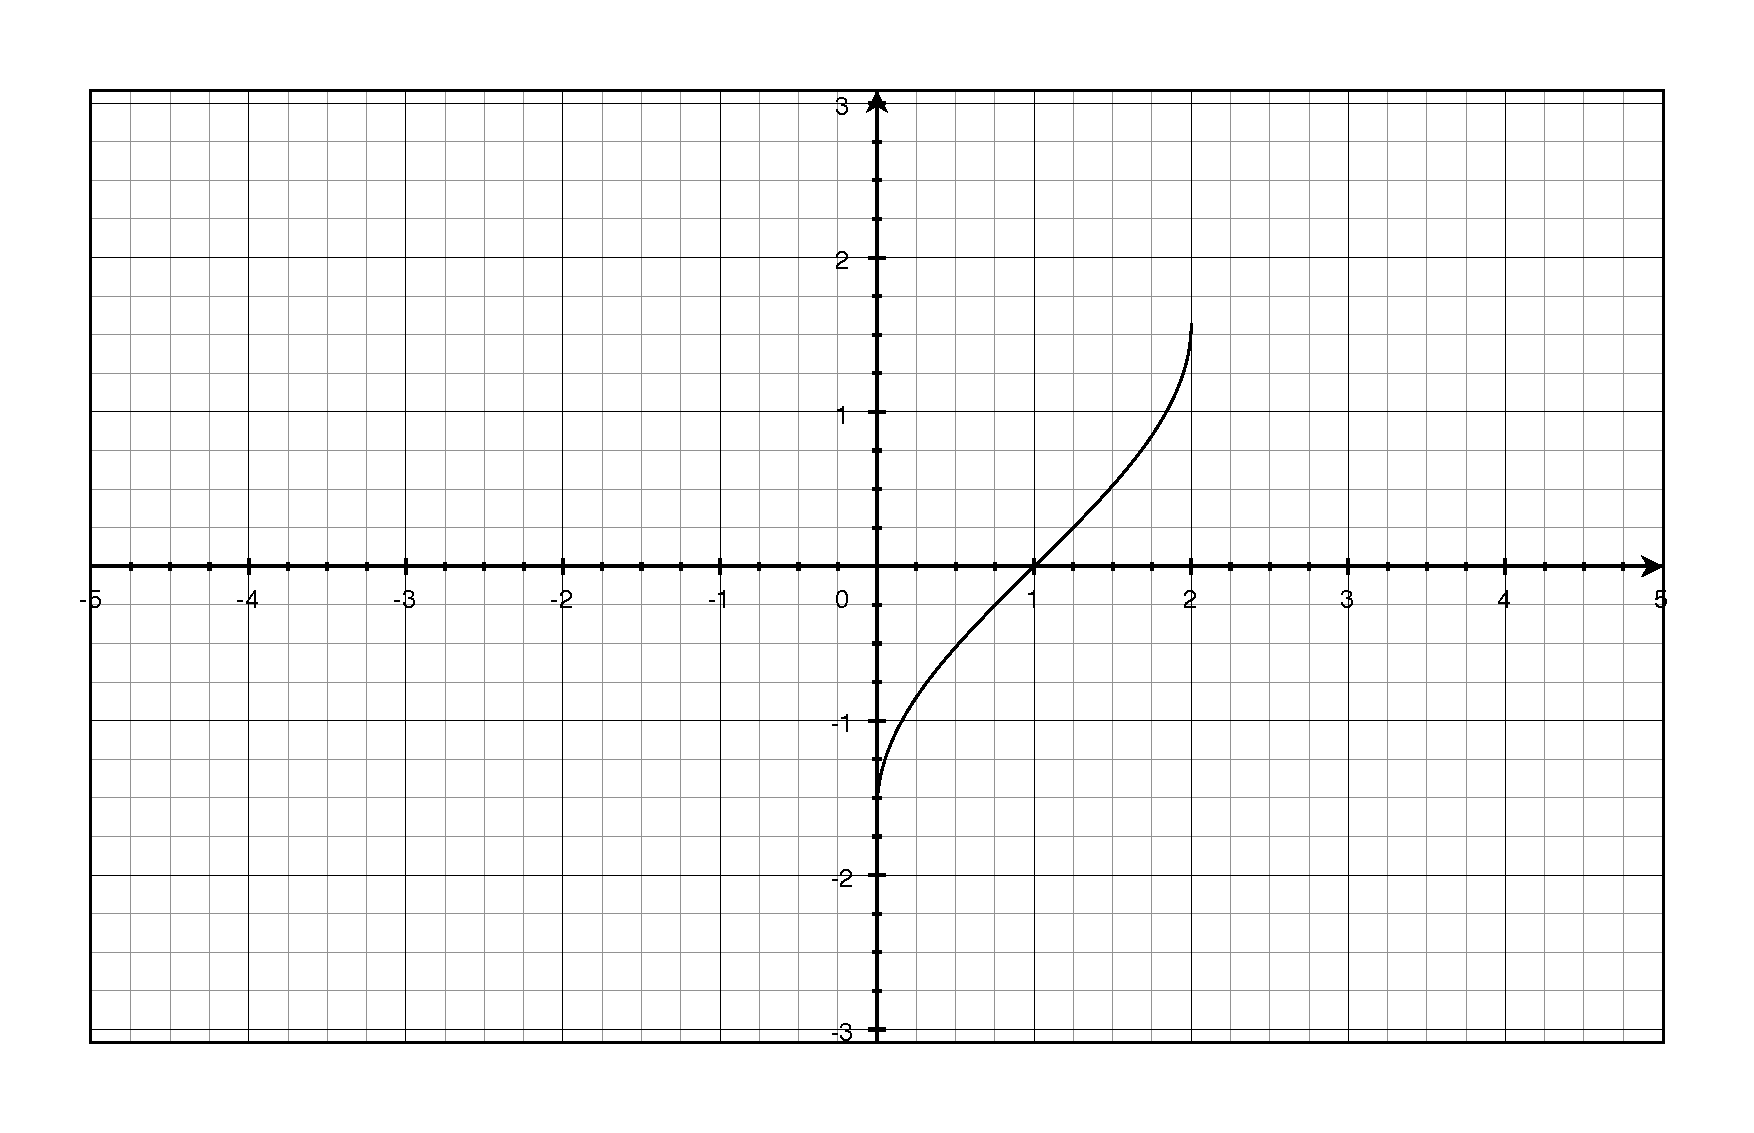
\includegraphics[scale=.3]{question_77.eps}
  \caption*{Question 77}
\end{figure}

\item[80] 
\begin{figure}[H]
  \centering
  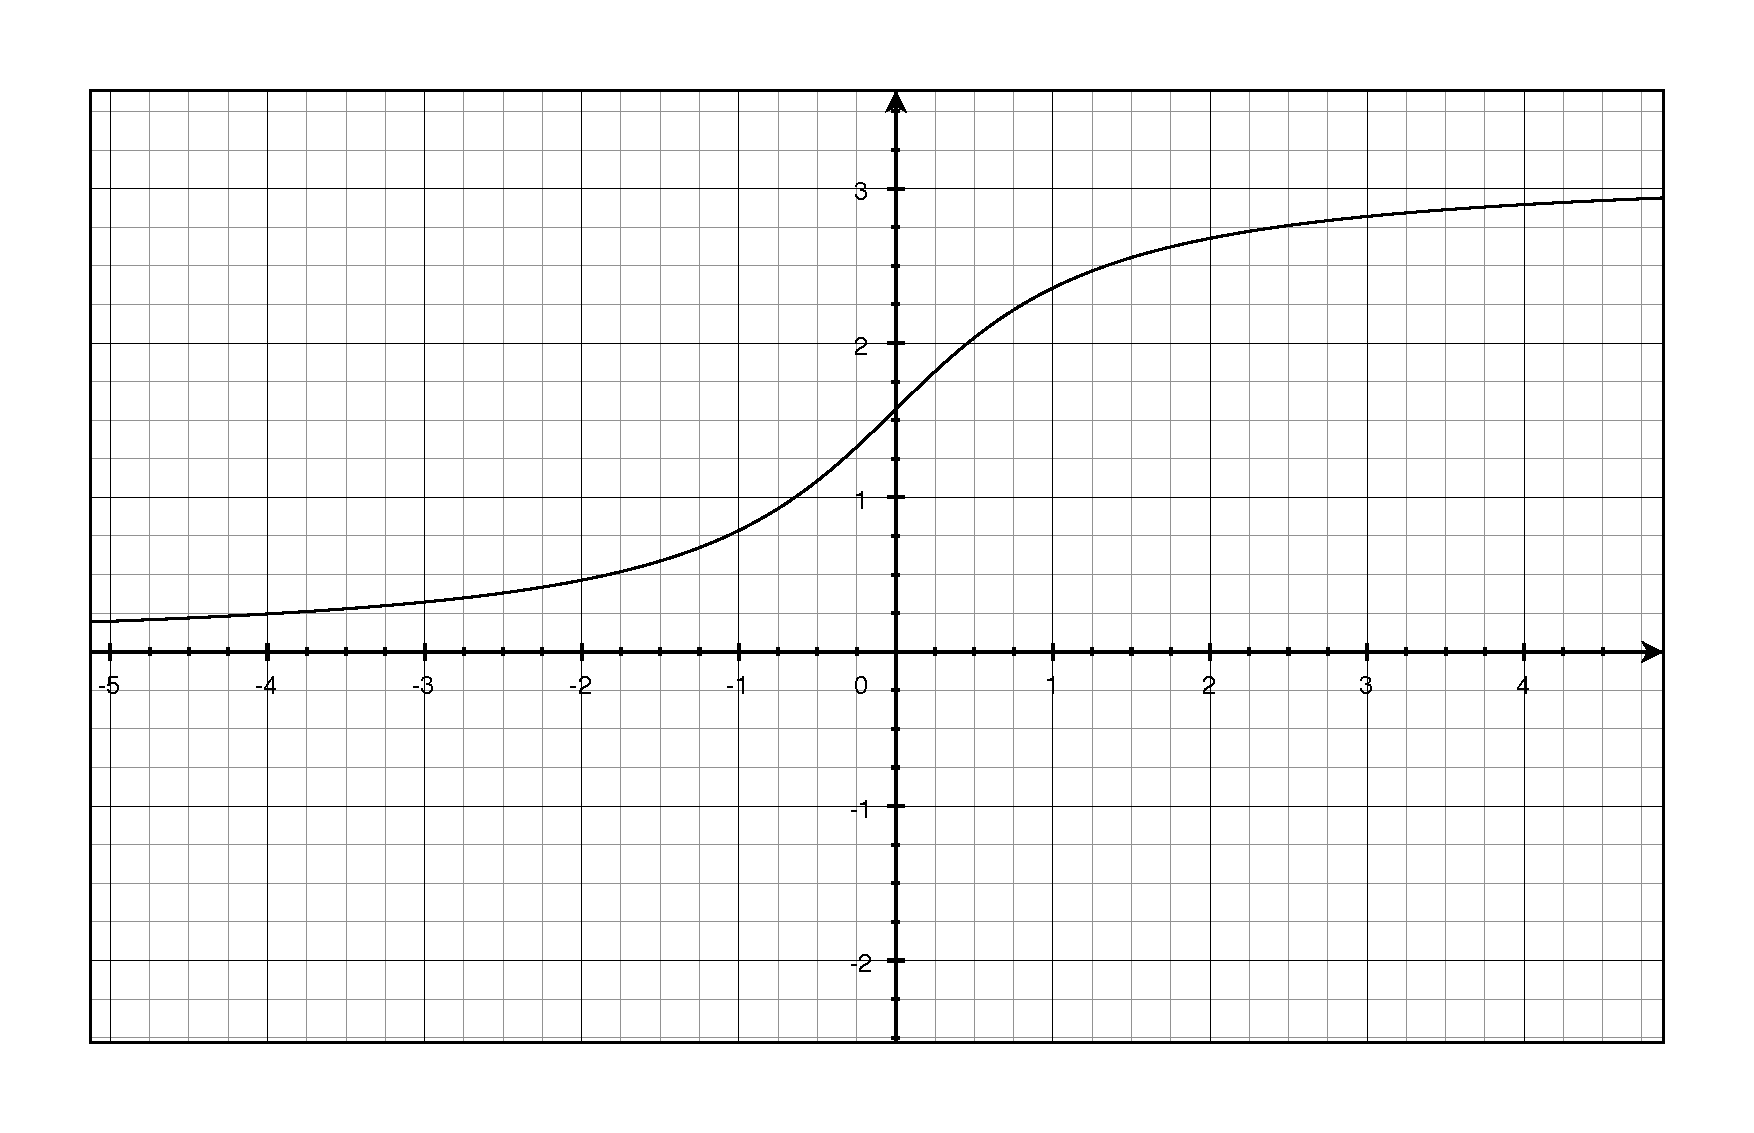
\includegraphics[scale=.3]{question_80.eps}
  \caption*{Question 80}
\end{figure}

\item[82] 
\begin{figure}[H]
  \centering
  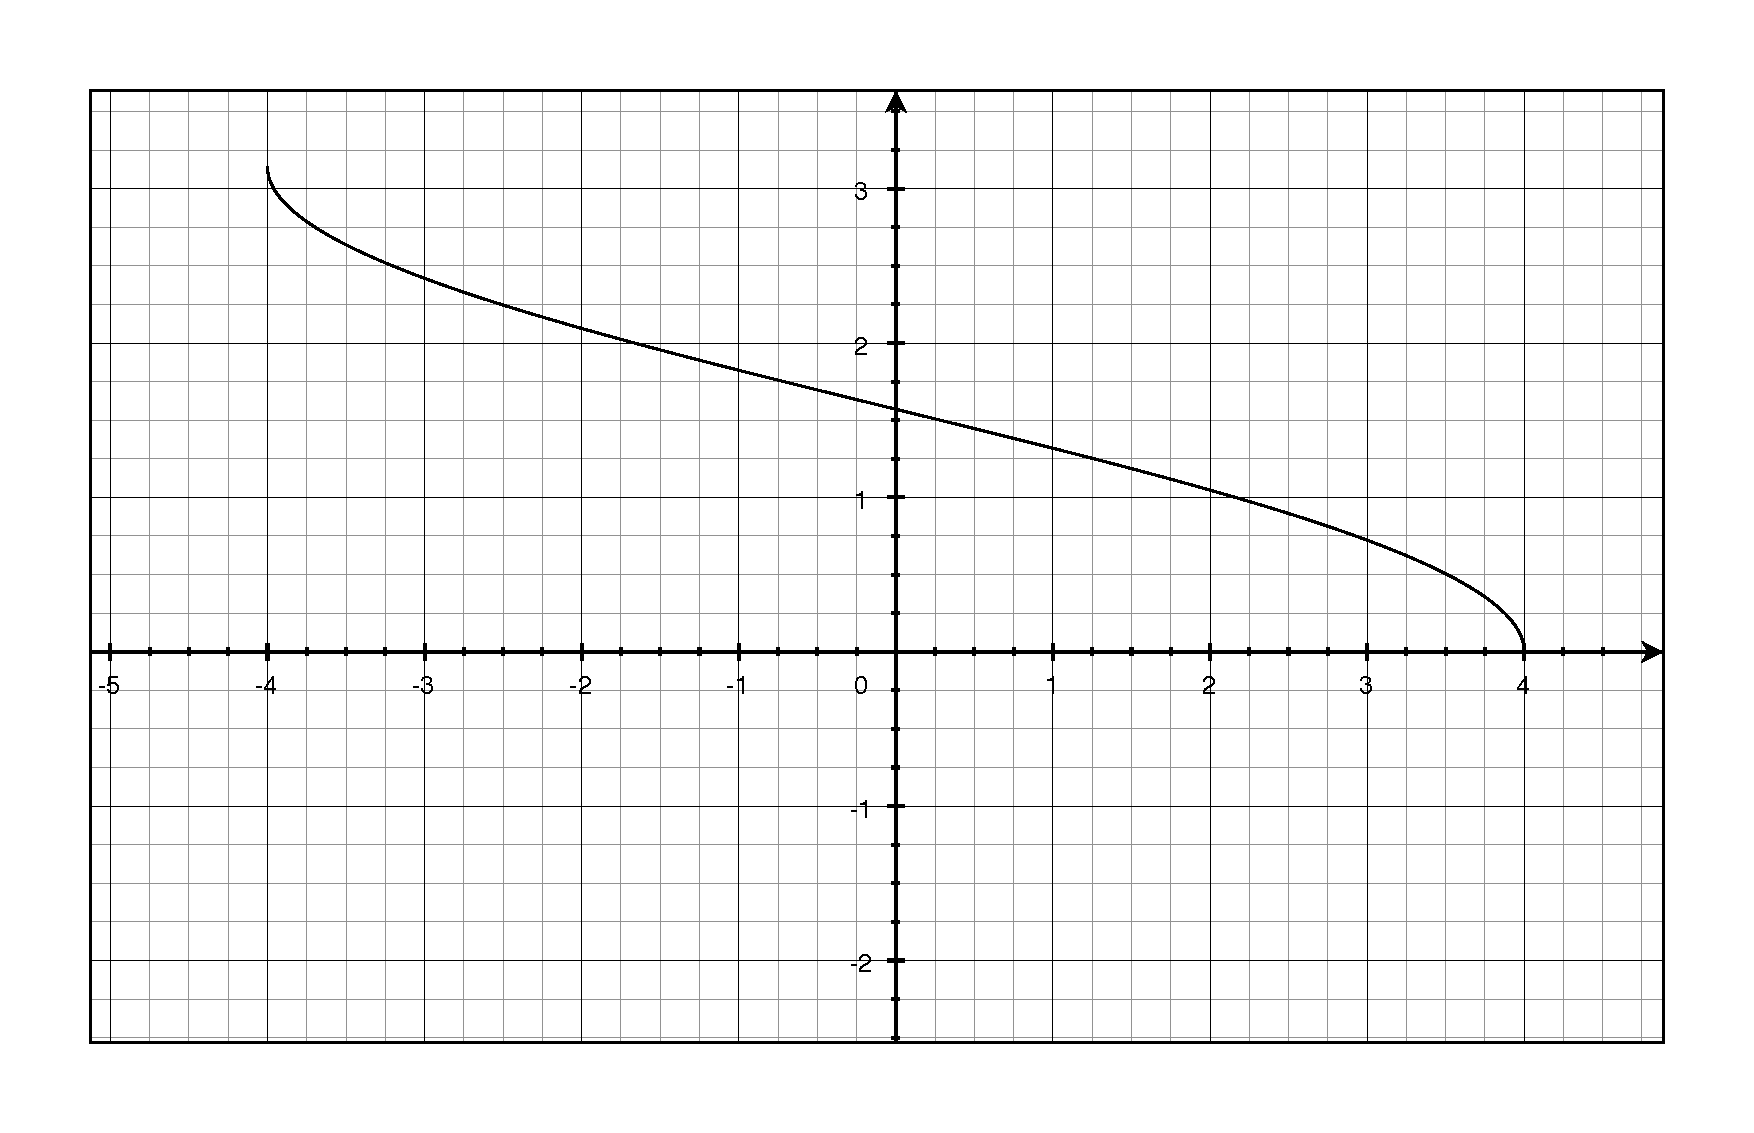
\includegraphics[scale=.3]{question_82.eps}
  \caption*{Question 82}
\end{figure}

\item[92]
\begin{description}

\item[a]
\[
  \theta(s) = \arctan \frac{s}{750} 
\]

\item[b]
\begin{itemize*}
  \item $\theta(300) = \arctan \dfrac{300}{750}  \approx 22 \degree$
  \item $\theta(1200) = \arctan \dfrac{1200}{750} \approx 58 \degree$
\end{itemize*}

\end{description}

\item[94]

\begin{description}
\item[a]
\[
  \theta(x) = \arctan \frac{6}{x}
\]

\item[b]
\begin{itemize*}
  \item $\theta(7) = \arctan \dfrac{6}{7} \approx 41 \degree$
  \item $\theta(1) = \arctan \dfrac{6}{1} \approx 81 \degree$
\end{itemize*}

\item[96]
false.  arcsin is in the range $\left[ -\dfrac{\pi}{2}, \dfrac{\pi}{2} \right]$ and $\arcsin \dfrac{1}{2} = \dfrac{\pi}{6}$

\item[97]
false.  arctan is in the range $\left[ -\dfrac{\pi}{2}, \dfrac{\pi}{2} \right]$ and $\arctan 1 = \dfrac{\pi}{4}$

\end{description}

\section{Pages 428-431}

\item[15]
\begin{align*}
  \tan 25 \degree &= \frac{50}{r} \\
  r &= \frac{50}{\tan 25 \degree} \\
  r &\approx 107 \text{ ft}
\end{align*}

\item[21]
\begin{align*}
  \sin 34 \degree &= \frac{d}{4000} \\
  d &= 4000 \sin 34 \degree \\
  d &\approx 2237 \text{ ft}
\end{align*}

\item[25]
The distance from the center of the earth to the satellite is the hypotenuse of the triangle: $h = 4000 + 12500 = 16500 \text{ miles}$.

The angle in the center of the diagram is the same as the angle of depression.  So the angle of depression is:
\[
  \theta = \arccos \frac{4000}{16500} \approx 76 \degree
\]

\item[27]
After one minute, the plane will have traveled $275 \cdot 60 = 16500 \text{ ft}.$  

In this time, it will have climbed: $16500 \cdot \sin 18 \degree \approx 5099 \text{ ft}$

\item[49]

\begin{align*}
  \cos 35 \degree &= \frac{10}{a} \\
  a &= \frac{10}{\cos 35 \degree} \\
    &\approx 12.2 \\
\end{align*}

\begin{align*}
  \tan 35 \degree &= \frac{b}{10} \\
  b &= 10 \tan 35 \degree \\
    &\approx 7 \\
\end{align*}

\end{description}


\else

\vspace{2.5 in}

\begin{em}
Schoenberg always complained that his American pupils didn't do enough work.  There was one girl in the class in
particular who, it is true, did almost no work at all.  He asked her one day why she didn't accomplish more.  She said,
``I don't have any time.''  He said, ``How many hours are there in the the day?''  She said, ``Twenty-four.''  He said,
``Nonsense: there are as many hours in a day as you put into it.''
\end{em}

\vspace{.2 cm}
\hspace{1.5 cm} --John Cage, {\em Indeterminacy}

\fi

\end{document}

